\section{实战Mnist}
\label{sec:mnist}

\begin{frame}
  \begin{center}
    \Huge{\textcolor{red}{实战Mnist}}
  \end{center}

  \begin{enumerate}
    \item \alert{提出问题}
    \item \alert{单层感知器}
    \item \alert{多层感知器}    
    \item \alert{调整超参}
    \item \alert{卷积神经网络}        
  \end{enumerate}   
\end{frame}

\subsection{提出问题}

\begin{frame}{图片:$ 28x28 = 784 $}
  \begin{figure}
    \centering
    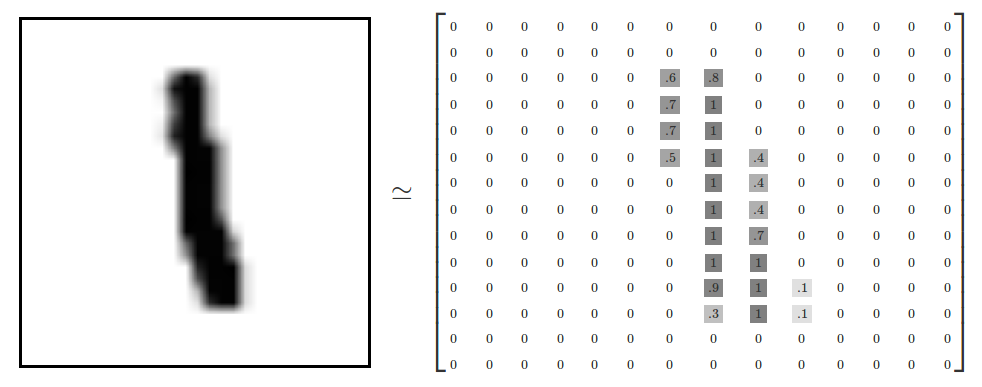
\includegraphics[width=0.8\textwidth]{mnist-x.png}
  \end{figure}
\end{frame}

\begin{frame}{训练数据集输入:$ [100(batch\_size), 784] $}
  \begin{figure}
    \centering
    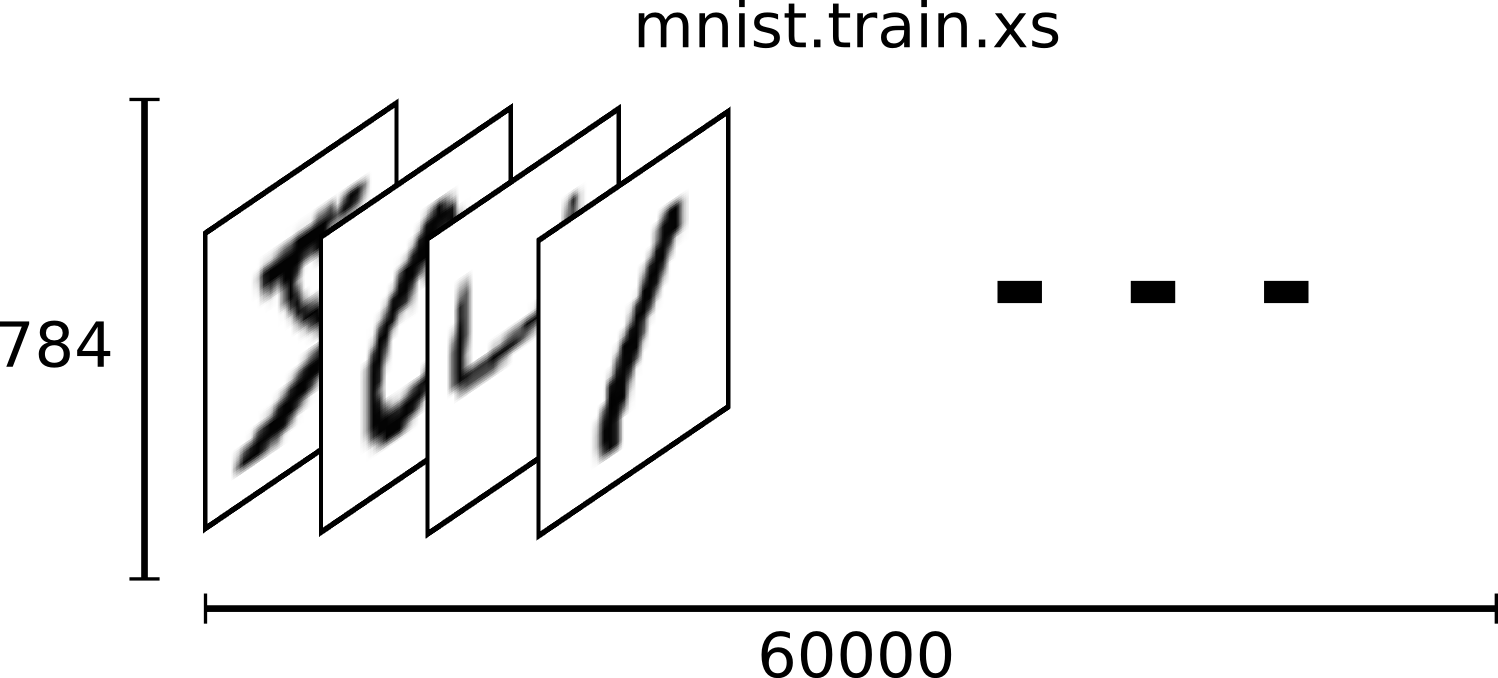
\includegraphics[width=0.8\textwidth]{mnist-train-xs.png}
  \end{figure}
\end{frame}

\begin{frame}{训练数据集输出:$ [100(batch\_size), 10] $}
  \begin{figure}
    \centering
    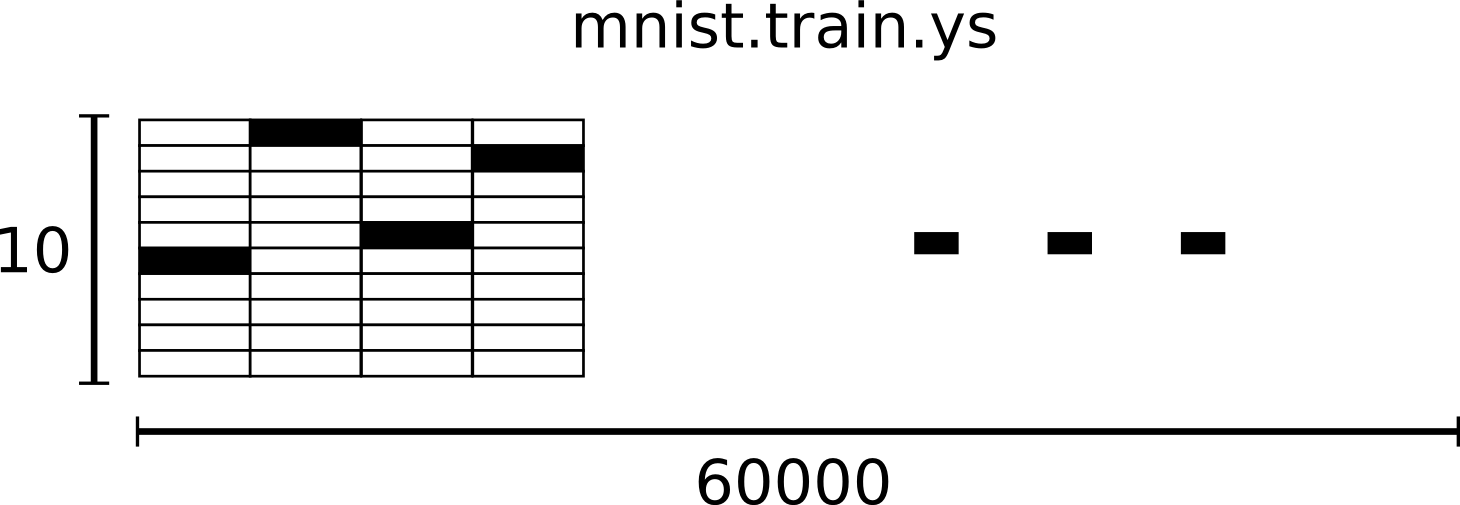
\includegraphics[width=0.8\textwidth]{mnist-train-ys.png}
  \end{figure}
\end{frame}

\subsection{单层感知器}

\begin{frame}{单层网络模型}
  \begin{figure}
    \centering
    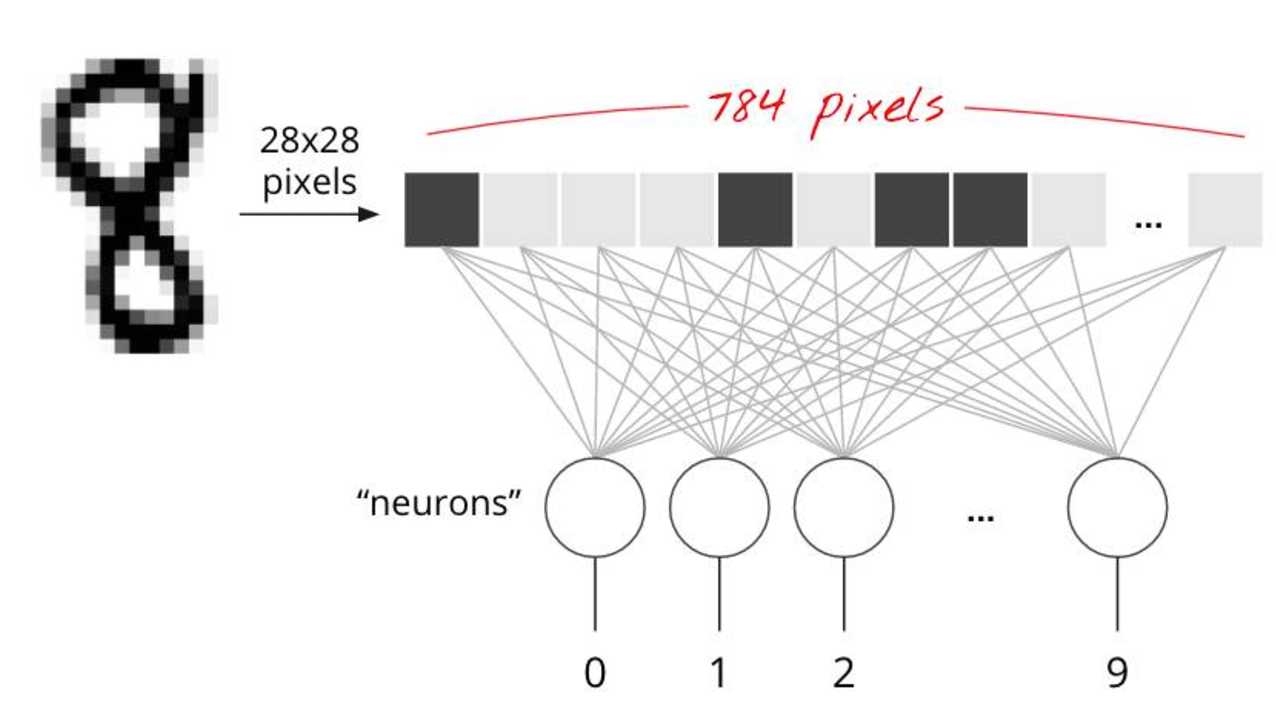
\includegraphics[width=0.8\textwidth]{mnist-slp.png}
  \end{figure}
\end{frame}

\begin{frame}[fragile]{占位符}
\begin{python}
# inputs
x  = tf.placeholder("float", [None, 784])  

# labels
t = tf.placeholder("float", [None, 10])
\end{python}

\begin{itemize}
  \item \code{tf.placeholder}定义了一个占位OP
  \item \code{None}表示未确定的样本数目(\code{batch\_size})
  \item \code{Session.run}时提供\code{feed\_dict}提供一个批次的样本数据
\end{itemize}
\end{frame}

\begin{frame}[fragile]{变量}
\begin{python}
# train parameters
W = tf.Variable(tf.zeros([784,10]))
b = tf.Variable(tf.zeros([10]))

# init\_op
init_op = tf.global_variables_initializer()
\end{python}

\begin{itemize}
  \item \alert{变量}:使用\code{tf.Variable}定义变量,常用于定义模型的权重和偏置
  \item \alert{初始化}:使用初始化\code{init\_op}初始化所有全局变量 
\end{itemize}
\end{frame}

\begin{frame}[fragile]{模型: 线性和}
  \begin{python}
y = tf.nn.softmax(tf.matmul(x, W) + b)
  \end{python}

  \begin{figure}
    \centering
    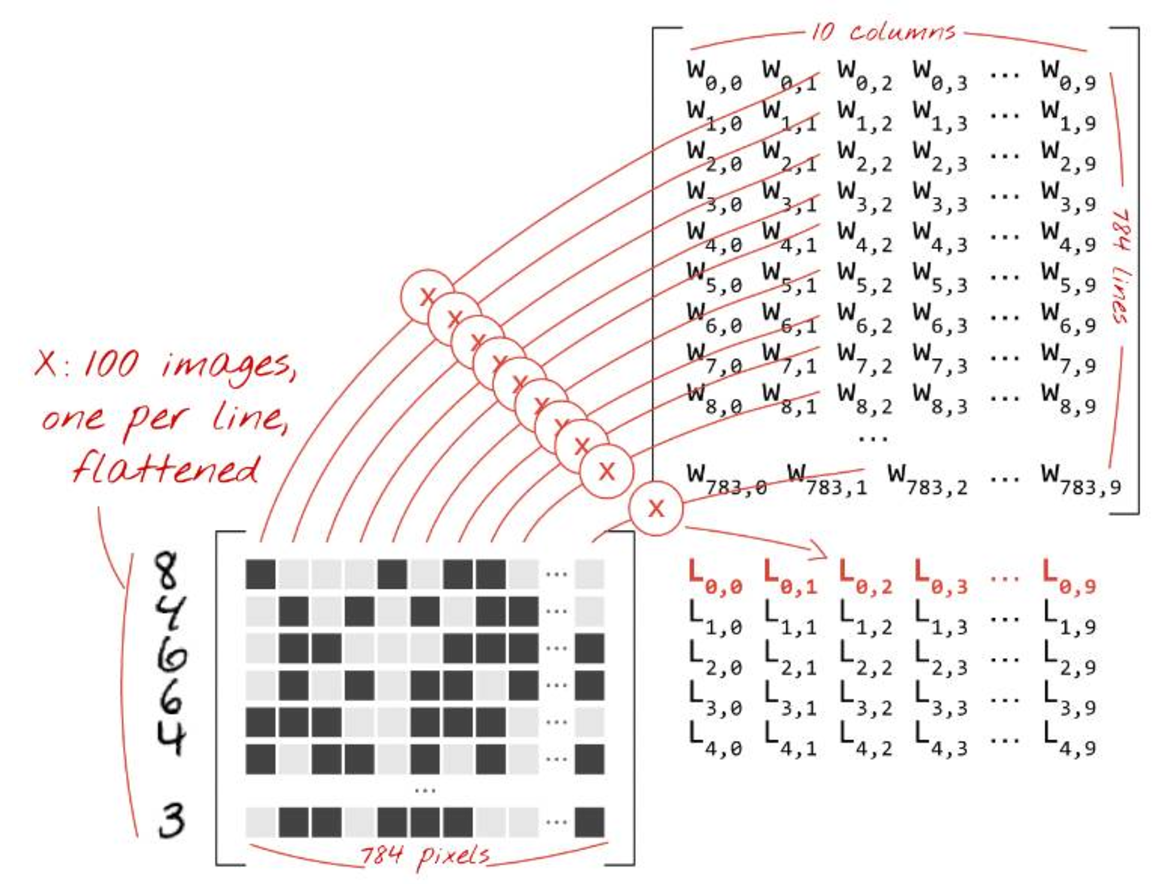
\includegraphics[width=0.6\textwidth]{mnist-linear-sum.png}
  \end{figure}
\end{frame}

\begin{frame}[fragile]{模型: Softmax}
  \begin{python}
y = tf.nn.softmax(tf.matmul(x, W) + b)
  \end{python}

  \begin{figure}
    \centering
    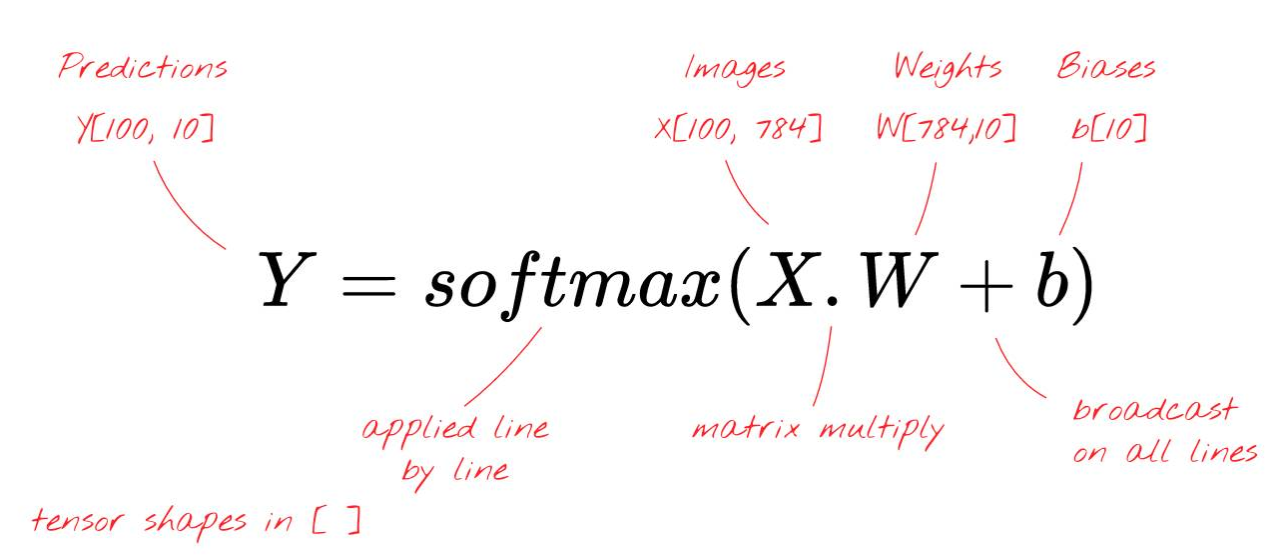
\includegraphics[width=0.8\textwidth]{mnist-softmax.png}
  \end{figure}
\end{frame}

\begin{frame}[fragile]{损失函数}
  \begin{python}
cross_entropy = -tf.reduce_sum(t * tf.log(y))
  \end{python}

  \begin{figure}
    \centering
    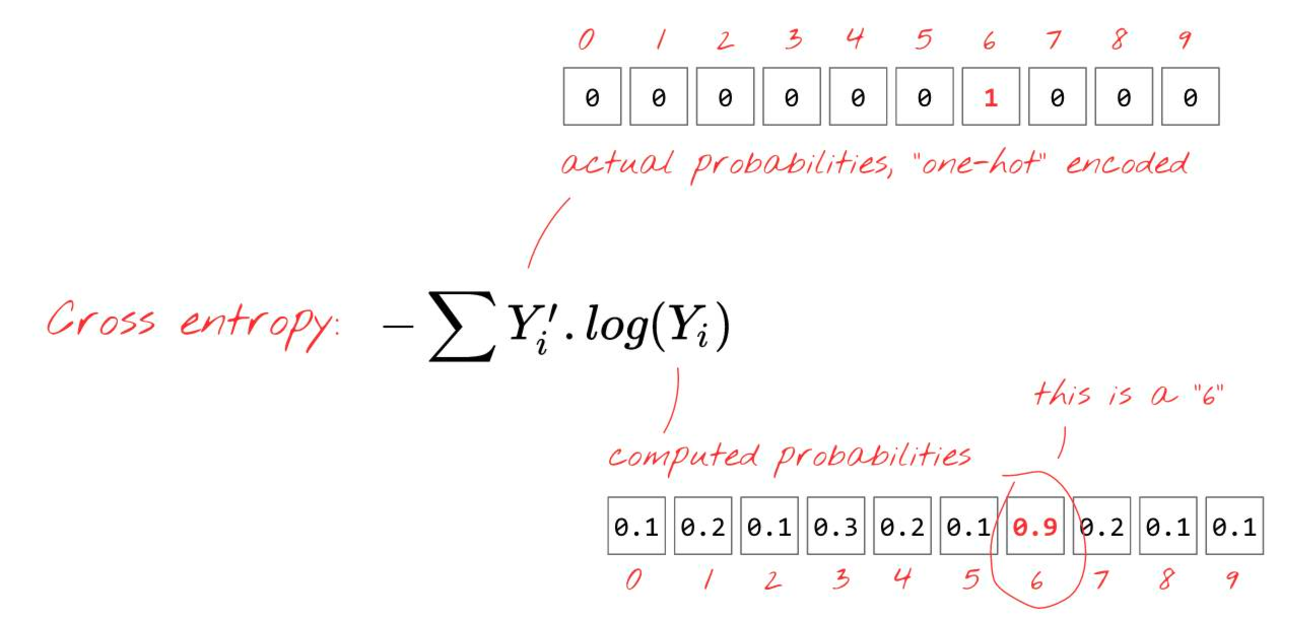
\includegraphics[width=0.8\textwidth]{mnist-cross-entropy.png}
  \end{figure}
\end{frame}

\begin{frame}[fragile]{执行训练}
\begin{python}
correct_prediction = tf.equal(tf.argmax(y, 1), tf.argmax(t, 1))
accuracy = tf.reduce_mean(tf.cast(correct_prediction, tf.float32))

with tf.Session() as sess:
  sess.run(init_op)

  for step in range(1000):
    batch_xs, batch_ys = mnist.train.next_batch(100)        
    sess.run(train_step, feed_dict={x: batch_xs, t: batch_ys})

    if step % 10 == 0:
      acc, loss = sess.run([accuracy, cross_entropy], 
        feed_dict={x: batch_xs, t: batch_ys})
    
    if step % 100 == 0:
      acc, loss = sess.run([accuracy, cross_entropy], 
        feed_dict={x: mnist.test.images, t: mnist.test.labels}) 
\end{python}
\end{frame}

\begin{frame}[fragile]{精度:约为92\%}
  \begin{figure}
    \centering
    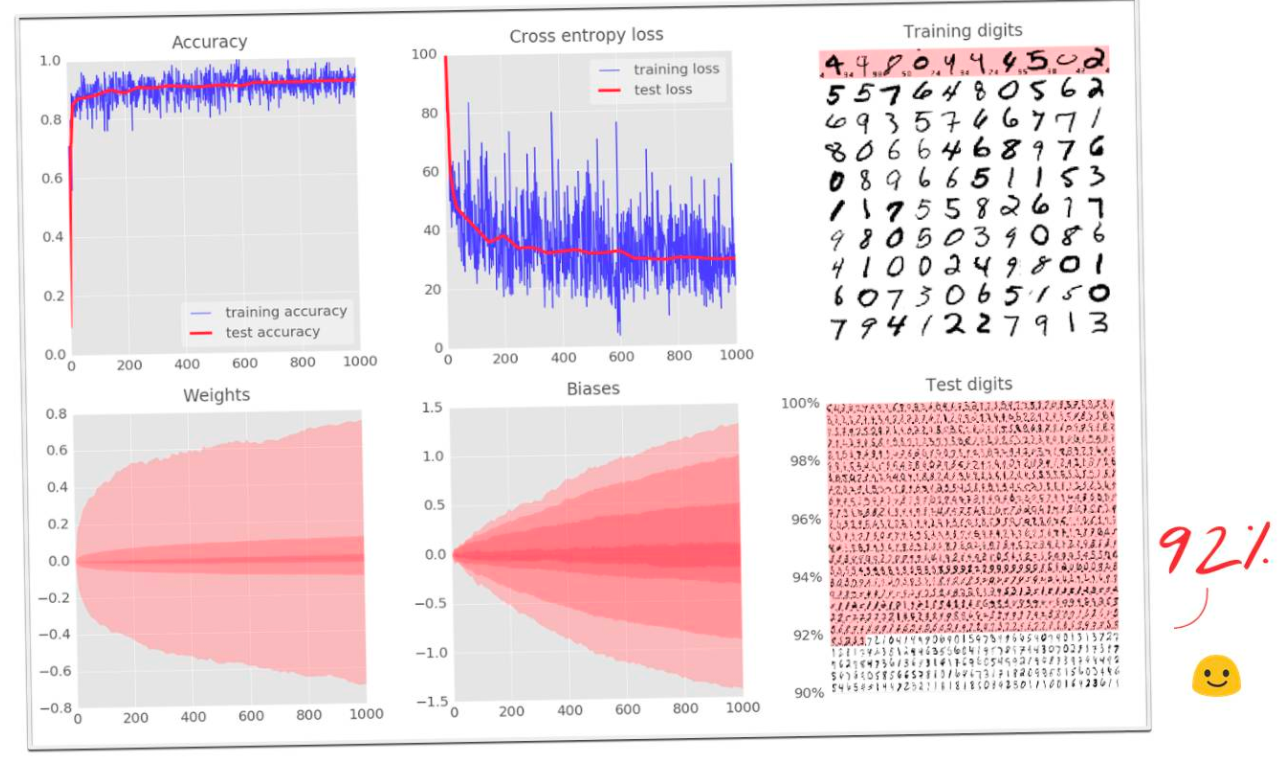
\includegraphics[width=0.9\textwidth]{mnist-slp-accuracy.png}
  \end{figure}
\end{frame}



